\documentclass[12pt,a4paper, oneside]{report}
%\documentclass[12pt,a4paper, oneside]{extreport}


%%%%%%%%%%%%%%%%%%%%%%%% Шрифты %%%%%%%%%%%%%%%%%%%%%%%%%%%%%%%%%
\usepackage{fontspec}         % пакет для подгрузки шрифтов
\setmainfont{Arial}   % задаёт основной шрифт документа
\defaultfontfeatures{Mapping=tex-text}

\newfontfamily{\cyrillicfonttt}{Arial}
\newfontfamily{\cyrillicfont}{Arial}
\newfontfamily{\cyrillicfontsf}{Arial}

\usepackage{polyglossia}      % Пакет, который позволяет подгружать русские буквы
\setdefaultlanguage{russian}  % Основной язык документа
\setotherlanguage{english}    % Второстепенный язык документа
% Разные мелочи для русского языка из пакета babel
\setkeys{russian}{babelshorthands=true}

%%%%%%%%%% Работа с картинками %%%%%%%%%
\usepackage{graphicx}                  % Для вставки рисунков
\usepackage{graphics}
\graphicspath{{images/}{pictures/}}    % можно указать папки с картинками
\usepackage{wrapfig}                   % Обтекание рисунков и таблиц текстом


%%%%%%%%%% Графика и рисование %%%%%%%%%%
\usepackage{tikz, pgfplots}  % язык для рисования графики из latex'a


%%%%%%%%%% Гиперссылки %%%%%%%%%%
\usepackage{xcolor}              % разные цвета

% Два способа включить в пакете какие-то опции:
%\usepackage[опции]{пакет}
%\usepackage[unicode,colorlinks=true,hyperindex,breaklinks]{hyperref}

\usepackage{hyperref}
\hypersetup{
    unicode=true,           % позволяет использовать юникодные символы
    colorlinks=true,       	% true - цветные ссылки, false - ссылки в рамках
    urlcolor=blue,          % цвет ссылки на url
    linkcolor=black,          % внутренние ссылки
    citecolor=green,        % на библиографию
	pdfnewwindow=true,      % при щелчке в pdf на ссылку откроется новый pdf
	breaklinks              % если ссылка не умещается в одну строку, разбивать ли ее на две части?
}

\usepackage{csquotes}            % Еще инструменты для ссылок

%%%%%%%%%% Другие приятные пакеты %%%%%%%%%
\usepackage{multicol}       % несколько колонок
\usepackage{verbatim}       % для многострочных комментариев

\usepackage{enumitem} % дополнительные плюшки для списков
%  например \begin{enumerate}[resume] позволяет продолжить нумерацию в новом списке

\usepackage{todonotes} % для вставки в документ заметок о том, что осталось сделать
% \todo{Здесь надо коэффициенты исправить}
% \missingfigure{Здесь будет Последний день Помпеи}
% \listoftodos --- печатает все поставленные \todo'шки



%%%% Оформление %%%%%%%
\usepackage[14pt]{extsizes} % Возможность сделать 14-й шрифт

% размер листа бумаги
\usepackage[paper=a4paper,top=10mm, bottom=10mm,left=35mm,right=35mm,includefoot,includehead]{geometry}

%\usepackage{indentfirst}       % установка отступа в первом абзаце главы!!!

\usepackage{setspace}
\setstretch{1}  % Межстрочный интервал
\setlength{\parindent}{0em} % Красная строка.
\setlength{\parskip}{4mm}   % Расстояние между абзацами
% Разные длины в латехе https://en.wikibooks.org/wiki/LaTeX/Lengths

\flushbottom                            % Эта команда заставляет LaTeX чуть растягивать строки, чтобы получить идеально прямоугольную страницу
\righthyphenmin=2                       % Разрешение переноса двух и более символов
\widowpenalty=300                     % Небольшое наказание за вдовствующую строку (одна строка абзаца на этой странице, остальное --- на следующей)
\clubpenalty=3000                     % Приличное наказание за сиротствующую строку (омерзительно висящая одинокая строка в начале страницы)
\tolerance=1000     % Ещё какое-то наказание.
\usepackage{nameref}

\usepackage{fancyhdr} % Колонтитулы
\pagestyle{fancy}

\renewcommand{\headrulewidth}{0.2pt}  % Толщина линий, отчеркивающих верхний
	\lhead{ПРИЛОЖЕНИЕ \Asbuk{section}}
	\chead{\nameref{\thesection}}
	\rhead{\thepage}
	\cfoot{\newsize{  \href{http://vhogwarts.ru/}{Школа Чародейства и Волшебства <<Хогвартс>>} }} 
\usepackage{titlesec}  

% В Linux этот пакет сделан косячно. Исправляет это следующий непонятный кусок кода. 
\makeatletter
\patchcmd{\ttlh@hang}{\parindent\z@}{\parindent\z@\leavevmode}{}{}
\patchcmd{\ttlh@hang}{\noindent}{}{}{}
\makeatother
% Все куски кода ниже - понятные!
\titleformat{\chapter}
{\Huge\bfseries}
{Глава \thechapter-}{0.1 em}{} 
% В последних скобочках к каждой главе можно что-нибудт приписать.

% Убирает чеканутые отступы перед главами 
\titlespacing{\chapter}{0pt}{-20pt}{30pt} 
%{отступ слева}{отступ сверху}{отступ снизу}

\titleformat{\section}
{\bfseries\Large}
{\thesection}{0.5 em}{}

\titleformat{\subsection}
{\bfseries\large}
{\thesubsection}{0.5 em}{}


\newfontfamily\myfont{OlgaCTT}

\usepackage{afterpage}  % Пакет, который позволяет настраивать параметры отдельной страницы
\renewcommand{\thesection}{Приложение \Asbuk{section}:}
\newcommand{\newsize}[1]{{\fontsize{12}{1}\selectfont #1 }}
\begin{document}
	
\pagestyle{empty}

\begin{figure}
	\centering
	
\includegraphics[height=6cm, width=5cm]{hgw.png}
\end{figure}
		
\vspace{1cm}

\newsize{ Мистеру Денисову } 
			
\vspace{2.5cm}

Дорогой мистер Денисов! 
			
Мы рады проинформировать Вас, что Вам предоставлено место в Школе чародейства и волшебства <<Хогвартс>>. Пожалуйста, ознакомьтесь с приложенным к данному письму списком необходимых предметов и книг. 
			
Занятия начинаются 1 сентября. Ждем Вашу сову не позднее 31 июля. 
			
Искренне Ваша,


\newenvironment{hfont}{\myfont}{\par}
\begin{hfont}
{\fontsize{20}{1}\selectfont Minerva McGonagall}
\end{hfont}
			
Минерва МакГонагалл \\ заместитель директора
		

\vfill
\begin{center}
Школа Чародейства и Волшебства <<Хогвартс>>  

\newsize{ Директор: Альбус Дамблдор \\ \textit{ (Кавалер ордена Мерлина I степени, Великий волшебник, Верховный чародей, Президент Международной конфедерации магов)} }
\end{center}	


\newpage
\pagestyle{fancy}
\renewcommand{\labelitemi}{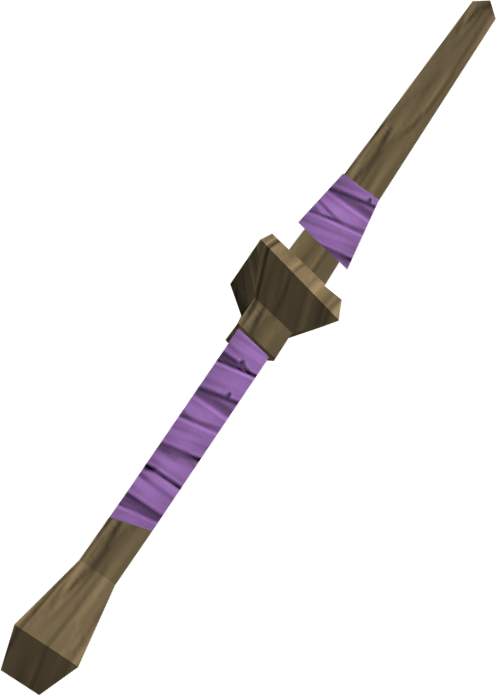
\includegraphics[scale=0.018]{mwand.png}}
\section{Список книг и предметов}\label{\thesection}
\textbf{Студентам-первокурсникам требуется:}
Форма:
\begin{itemize}
	\item Три простых рабочих мантии (черных).
	\item Одна простая остроконечная шляпа (черная) на каждый день.
	\item Одна пара защитных перчаток (из кожи дракона или аналогичного по свойствам материала).
	\item Один зимний плащ (черный, застежки серебряные).
\end{itemize}
\textbf{Также полагается иметь:} 
\begin{itemize}
	\item волшебную палочку 
	\item котел (оловянный, стандартный размер № 2)
	\item комплект стеклянных или хрустальных флаконов 
	\item телескоп 
	\item медные весы
\end{itemize}
\textit{Пожалуйста, не забудьте, что на одежду должны быть нашиты бирки с именем и фамилией студента}

\textbf{Каждому студенту полагается иметь следующие книги:}
\begin{itemize}
	\item «История магии». Батильда Бэгшот
	\item «Фантастические звери: места обитания». Ньют Саламандер
	\item «Курсическая книга заговоров и заклинаний» (первый курс).
	\item «Пособие по трансфигурации для начинающих». 
	\item «Тысяча магических растений и грибов».
	\item «Магические отвары и зелья». 
\end{itemize}

\newpage

\section{Список изучаемых предметов}\label{\thesection}
\textbf{На первом курсе будут изучаться следующие предметы:}
\begin{itemize}
	\item История магии
	\item Заклинания
	\item Трансфигурация
	\item Зельеваренье
	\item Случайные процессы с Демешевым Б.Б. 
\end{itemize}

\end{document}